\documentclass[useAMS,usenatbib]{mn2e}


\usepackage{times,graphicx,hyperref}
\usepackage{amssymb}
\usepackage[usenames, dvipsnames]{color}

\usepackage{lipsum}

%%%%% AUTHORS - PLACE YOUR OWN MACROS HERE %%%%%
\def\farcs{\hbox{$.\!\!^{\prime\prime}$}}
\def\farcsh{\hbox{$.\!^{\mathrm{s}}$}}
\def\mnras{MNRAS}
\def\nat{Nature}
\def\aap{A\&A}
\def\apj{ApJ}
\def\apjl{ApJ}
\def\aj{AJ}
\def\pasj{PASJ}
\def\pasp{PASP}
\def\apjs{ApJS}
\def\aaps{A\&AS}
\def\aplett{ApL}
\def\pasa{PASA}

%%%%%%%%%%%%%%%%%%%%%%%%%%%%%%%%%%%%%%%%%%%%%%%% 

\title[Globular clusters in Maffei 1]{A wide-field study of globular
  clusters in the nearest giant elliptical: Subaru/Suprime-Cam
  observations of Maffei 1\thanks{Based on data collected at Subaru
    Telescope, which is operated by the National Astronomical
    Observatory of Japan.}}  

\author[S. Hinton et al.]{
Samuel Hinton$^{1,2}$, 
Ricardo Salinas$^{3}$% \thanks{E-mail: rsalinas@gemini.edu}, 
Aaron J. Romanowsky$^{4,5}$, and maybe some others
\\
$^1$School of Mathematics and Physics, University of Queensland, QLD 4072, Australia \\
$^2$Australian Astronomical Observatory, North Ryde, NSW 2113, Australia \\
$^3$Gemini Observatory\\ 
$^4$Department of Physics \& Astronomy, San Jos\'e
  State University, San Jose, CA 95192, USA\\ 
$^5$University of California Observatories,
1156 High Street, Santa Cruz,CA 95064, USA
}
\begin{document}

\date{Accepted ... Received ...; in original form ...}


\pagerange{\pageref{firstpage}--\pageref{lastpage}} \pubyear{2016}

\maketitle

\label{firstpage}
%%%%%%%%%%%%%%%%%%%%%%%%%%%%%%%%%%%%%%%%%%%%%%%

\begin{abstract}
Lorem ipsum dolor sit amet, consectetur adipiscing elit. Sed condimentum ipsum faucibus sem elementum, eu consectetur risus consectetur. Praesent quis aliquam risus. Vivamus interdum et eros gravida rhoncus. Proin accumsan finibus pellentesque. Praesent et erat eu velit maximus condimentum. Integer ornare vestibulum dolor nec pretium. Suspendisse suscipit, metus sed consectetur pretium, ligula nunc mollis quam, id dapibus est tortor et massa. Maecenas maximus elit orci, sit amet tincidunt libero ultrices a. Nullam sit amet condimentum libero. Duis ullamcorper lorem in nisi gravida tincidunt. Aliquam erat volutpat. Sed vitae sem a elit mattis porttitor.
\end{abstract}

\begin{keywords}
Galaxies: individual: Maffei 1 -- Galaxies: star clusters
\end{keywords}

%%%%%%%%%%%%%%%%%%%%%%%%%%%%%%%%%%%%%%%%%%%%%%%%
\section{Introduction}
\label{sec:intro}

{\bf Add some general remarks on globular cluster systems.}
 
Maffei 1 is a giant elliptical galaxy \citep{maffei68,spinrad71}
located at only 0.5\degr\,North of the Galactic plane. This position
implies large obscuration by dust from the Galactic disc which has
hampered the measurement of even the most basic parameters of the
galaxy.

{\bf Give main results from the literature}

Its particular relative position has also conspired against the study
of its globular clusters (GCs). Studies of its globular cluster system
(GCS) have produced only a handful of GC candidates
\citep{davidge02,buta03,davidge05}, whereas for its luminosity
\citep[$M_V\sim-20.80$,][]{fingerhut07}, the size of its GCS should be
comparable to the one of Cen A, hosting $\sim 1300$ GCs
\citep{harris10}. 

In this paper we present the first wide-field study of the Maffei 1
GCS system using Subaru/SuprimeCam imaging.In Sect. \ref{sec:obs} we
present the imaging data used, as well as its reduction and
photometry. In Sect. \ref{sec:results} we present the GCs selection,
together with the derived properties of the
GCS. Sect. \ref{sec:discussion} puts our results on a wider context,
while Sect. \ref{sec:conclusions} summarizes the work and give
conclusions.

%%%%%%%%%%%%%%%%%%%%%%%%%%%%%%%%%%%%%%%%%%%%%%%%%%%%%%%%%%%%%%%%%%%%
\section{Subaru/Suprime-Cam observations and data reduction}
\label{sec:obs}



Maffei 1 images were obtained using Suprime-Cam \citep{miyazaki02}
located on the Subaru telescope, Mauna Kea, Hawaii. Suprime-Cam
comprises 10 CCD detectors separated by $\sim15\arcsec$ covering a
field-of-view of $34\arcmin\times27\arcmin$ with a pixel scale of
0.2\arcsec. SDSS $r'$, $i'$ and $z'$-band images were obtained during
the night of January 5th, 2011.  Several short exposures were taken
with a $\sim\!  1\arcmin$ dither pattern, totalling 385, 280, and 280
seconds in the $r'$, $i'$ and $z'$-bands, respectively.

Suprime-Cam images reduction was conducted within the \textsc{sdfred2}
pipeline \citep{ouchi04}. Reduction steps include bias subtraction,
flat-fielding, correction for atmospheric distortions, point spread
function (psf) equalization (i.e. the normalization of the psf to a
single shape across the detectors and exposures), sky subtraction,
image alignment and finally, the combination of all exposures and
detectors into single images. Final averaged images have a
field-of-view of $\sim37\arcmin\times 31\arcmin$ and a seeing quality
of 0.72\arcsec, 0.68\arcsec and 0.63\arcsec, for $r'$, $i'$ and $z'$,
respectively. The field of view in $z'$ is shown in Figure \ref{fig:maffei1}, and a detailed colour image of the galactic core is presented in Figure \ref{fig:maffei1colour}.

For the $z'$ image set, which is used as the basis for the GC
candidates identification given its higher image quality (see
Sect. \ref{sec:gc_candidates}), a parallel alternative reduction
process was adopted. The $z'$ dataset not only provides the reddest
band to pierce through the Galactic plane, but also contains the best
seeing images. Even though the same \textsc{sdfred2} pipeline was
mostly used, a couple of the aforementioned reduction steps were
skipped in order to maintain image manipulations that could alter the
image quality to a minimum. Firstly, given the slight degradation of
the psf towards the outer detectors, psf equalization across the chips
would imply a lost of information on the best chips. For this reason
the detectors were reduced independently and not combined into a
single image as a final step. As a second difference, we did not apply
any correction for atmospheric distortions, since it resulted in an
increase of about 10\% of the measured stellar full width at half
maximum (fwhm) due to charge shifting to neighbor pixels. Finally,
images with psf sizes significantly larger than the mean were excluded
from the final image combination. This resulted in the rejection of
zero to two exposures per chip.

Coordinate transformations and image combination for the individual
detectors were carried out with \textsc{daomaster/montage2}
\citep{stetson93,stetson94}, which give more flexibility than
\textsc{sdfred2} for images with a small overlapping area. Measured
fwhm on the combined $z'$ images varies between 0.52\arcsec to
0.58\arcsec from detector to detector, which are noticeably better
than the 0.62\arcsec measured on the combined full frame image given
by \textsc{sdfred2}.

As a last step prior to initial photometry, images presenting large background
variations (containing Maffei 1 light or Galactic cirrus), were
median filtered with an annulus kernel, with outer radius size of 150 pixel and an inner radius of 105 pixels; a large size that preserves point-like sources unaltered. Photometry and astrometry were performed on the images fully processed with the \textsc{sdfred2} pipeline.

\begin{figure}
\includegraphics[width=0.49\textwidth]{images/ds9.jpeg}
\caption{The Maffei 1 field as seen by Subaru-SuprimeCam in $z'$. Image size
  is approximately $37\arcmin\times 31\arcmin$. North is up and East is
  to the left.}
\label{fig:maffei1}
\end{figure}

\begin{figure}
	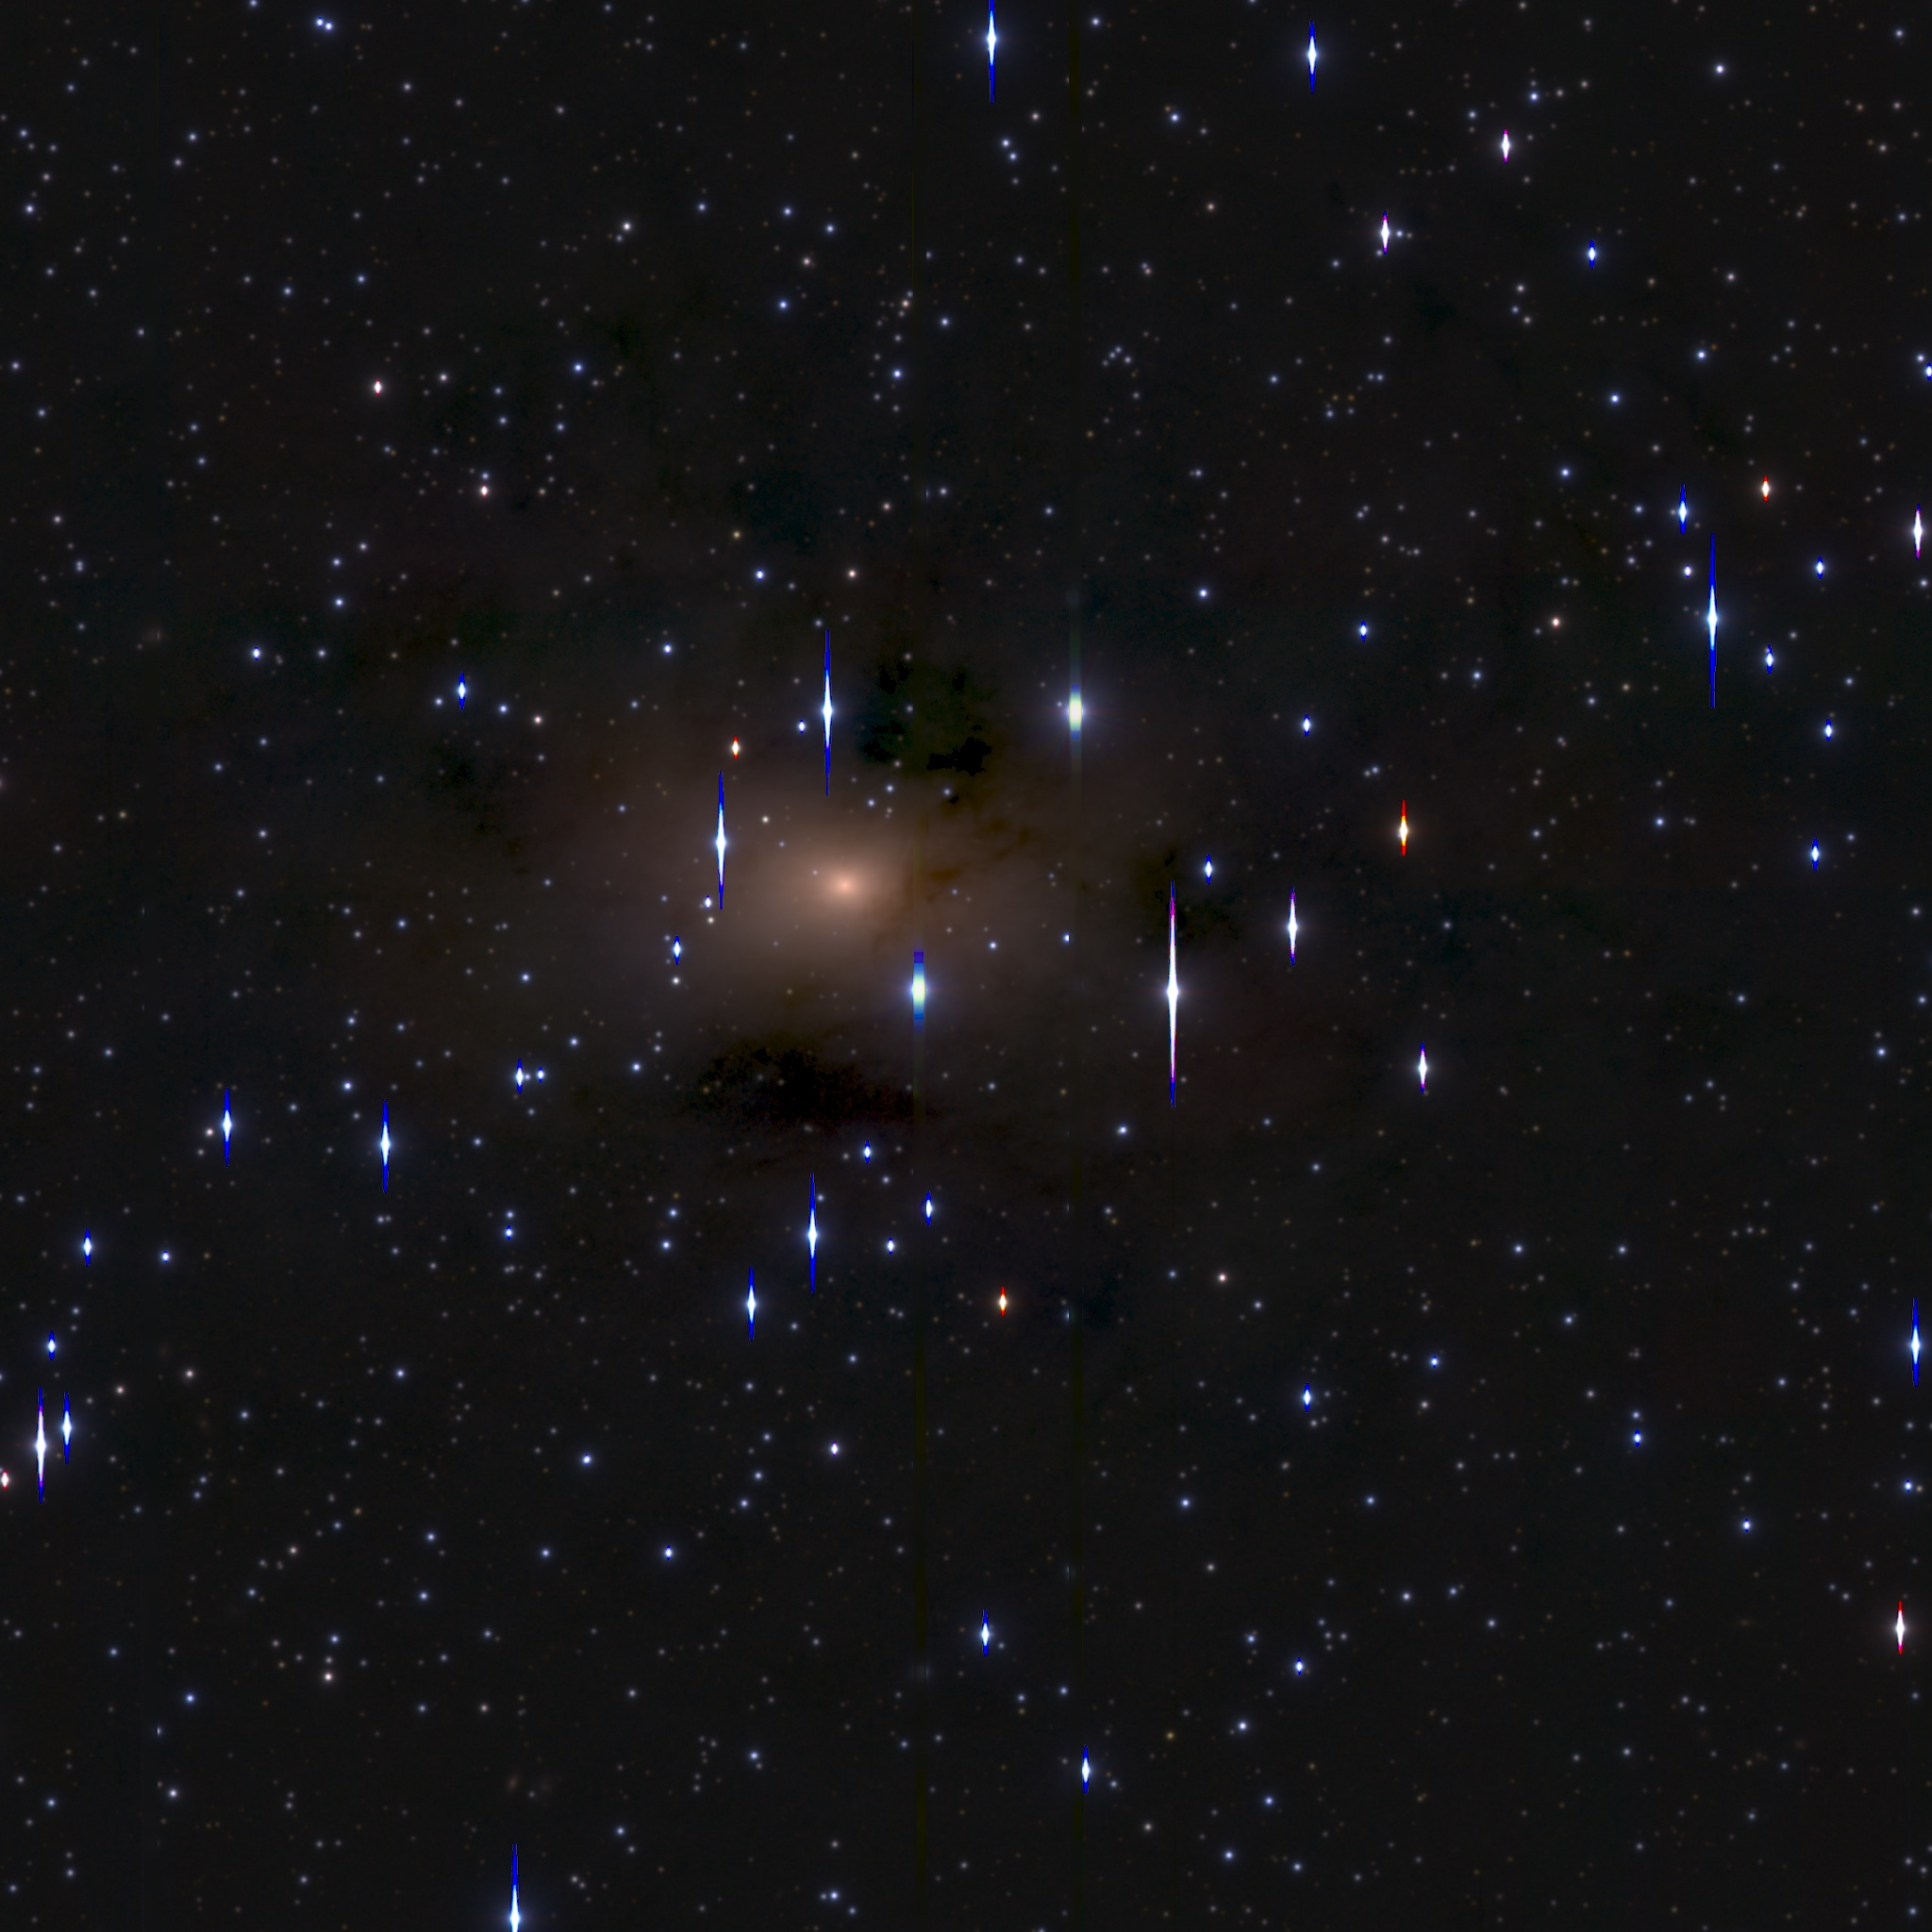
\includegraphics[width=0.49\textwidth]{images/center.jpg}
	\caption{The core of Maffei 1 shown in $z'$, $i'$ and $r'$, generated by \textsc{Stiff} \citep{bertin2012}. The image size is approximately $6.5\arcmin\times 6.5\arcmin$. North is up and East is to the left.}
	\label{fig:maffei1colour}
\end{figure}


\subsection{Stellar photometry}
\label{sec:photometry}


Manual aperture and psf-fitting photometry were carried out on a chosen
example tile using the
stand-alone \textsc{daophot2} photometric suite \citep{stetson87}. The
psf was modelled selecting $\sim$120--140\, bright and isolated stars
on each detector. A quadratically varying Moffat function was found to
provide the best description of the psf behaviour within the
detectors.

Photometry for all the sources was also obtained using
\textsc{SExtractor} \citep{bertin96}, which additionally provides
measurements of the size, orientation and ellipticity of the sources.

%%%%%%%%%%%%%%%%%%%%%%%%%%%%%%%%%%%%%%%%%%%%%%%%%%%%%%%%%%%%%%%%%%%%%%
\section{Results}
\label{sec:results}
\subsection{Selecting globular clusters candidates}
\label{sec:gc_candidates}

The basic selection criterion for GCs in Maffei 1 rests on the
non-stellar shape of their light profiles. This shape, usually smeared
out for distant systems or in images with low spatial resolution,
should be noticeable for the largest GCs in Maffei 1 given the
galaxy's distance and the quality of the imaging. A similar approach
has been applied successfully on ground-based imaging of GCs in the
slightly more distant elliptical galaxy Centaurus A
\citep{rejkuba01,gomez06,gomez07}. As manual inspection of all sources was infeasible
due to the number of sources, a machine learning approach was adopted in order
to differentiate between stellar sources and extended sources. Initially, the neural network
classifier contained inside \textsc{SExtractor} was utilised, but a posterior analysis has shown that clearly resolved sources have been assigned a \verb+CLASS_STAR+ parameter value as high
as 0.98, which on a blind approach would have been classified as
stars. Thus the algorithm was found to be insufficient ,and a new algorithm was developed. Training of the machine learning algorithms was performed by combining artificially generated data and manual classification on a single tile.

Manual classification was performed by visual analysis of the star-subtracted $z'$-image of the chosen CCD tile produced by the psf-fitting algorithm in
\textsc{allstar}. The image was were visually inspected to look for residuals that
revealed the presence of extended sources. The light profile of GCs
(but also galaxies) would be over-subtracted in the central parts and
under-subtracted in the wings, leaving an easily recognizable
``ring-shaped'' residual (see Fig. \ref{fig:subtraction}). A visual
inspection of the residuals in a tile is a
painstaking process, but provides benefit over only artificial data that does not model the full distribution of extendeds' properties accurately. Our selected approach revealed the presence of 77 extended sources in the Clarisse tile.

\begin{figure}
	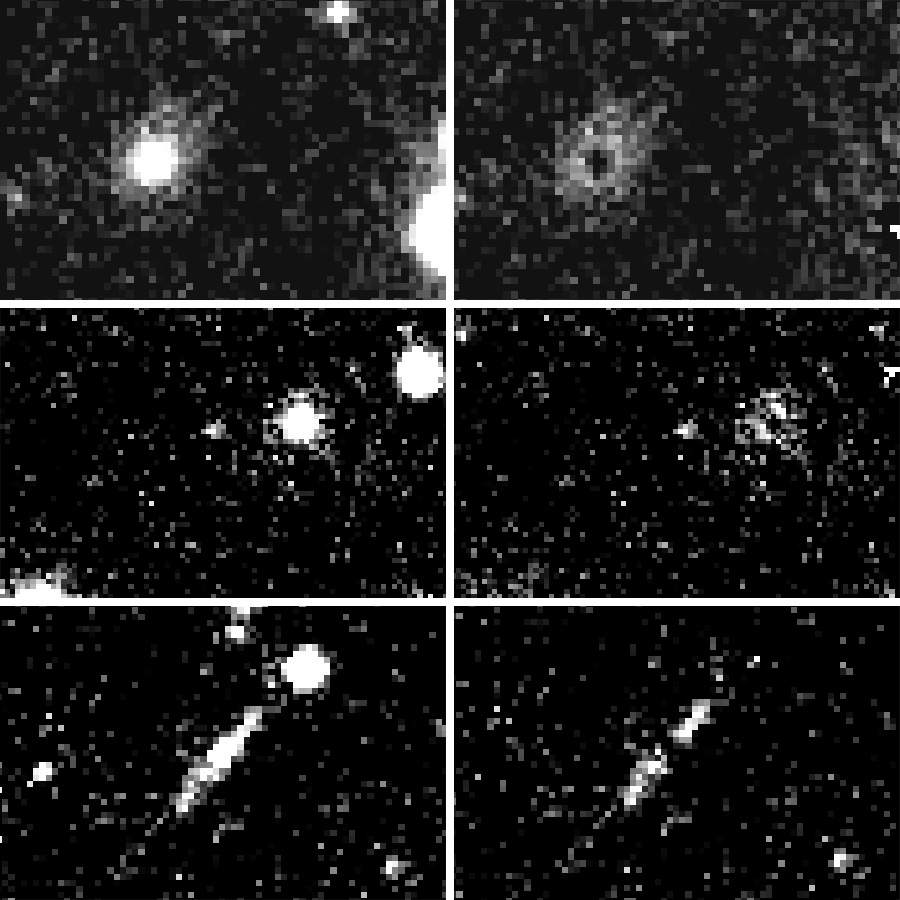
\includegraphics[width=0.49\textwidth]{images/Subtracted.jpg}
	\caption{Three examples of the psf-subtraction technique applied on the
		final $z$ images to reveal extended sources. The left panels show
		the original image, while the right panels are the psf-subtracted
		images. Top panels: A round object revealing a highly confident classification. Middle panels: A similar classification with a lower confidence due to the image noise. Bottom panels: An elongated extended object, in this case a galaxy viewed from the side, where the high ellipticity of the source allows differentiation between globular cluster and galaxy.}
	\label{fig:subtraction}
\end{figure}



Artificial stars and extended sources were added to the Clarisse tile by the use of the \verb|mksynth| task in \textsc{BAOlab} \citep{Larsen1999}. The psf input into the \verb|mksynth| function was determined using by automatically selecting a number of candidate psf stars (based on flux criterion, star classification and source isolation), and generating a subsampled psf using the \verb|digiphot| package in \textsc{iraf} {\color{red} CITE}. For generation of artificial extended objects, the \verb|mkcmppsf| task was also used to generate a compositie psf with a King model \citep{King1962} with concentration index of 30. The fwhm of the model was randomised to allow variation in the size of the artificial globular clusters. Both stars and extendeds were generated with uniform randomised magnitudes. The input data set was then created by using \textsc{SExtractor} to detect source properties of both the artificial sources and manually classified sources. In total, over $17\,000$ artifical globular cluster candidates and $170\,000$ artificial stars were introduced over a series of 300 artificial images to create a large set of data. The weighting of the manually detected stars and extended objects from the original tile was increased by a factor of a hundred to reflect their realism over artificial sources.

The input data was split into training, testing and validation sets, using ratios 0.4, 0.35 and 0.25 respectively, where multiple machine learning algorithms were trained on the training data, and the algorithm with the highest Matthews correlation coefficient\citep{matthews1975comparison} when evaluated on the validation set was selected as the final algorithm. The Matthews correlation coefficient was chosen to be maximised over other coefficients such as classifier accuracy, due to its fairness in dealing with unbalanced classes \citep{Baldi2000, Jurman2012}, which we expect to find with the number of point sources far exceeding the number of extended sources. Expected performance of the algorithm was determined by fitting to the test data set, and the probability of correctly classifying an extended object as a function of half light radius and magnitude is shown in Figure \ref{fig:comp1}.

The extended candidates for each tile given by the initial machine learning algorithm were then processed through the task \verb|iShape|, a procedure in the \textsc{BAOlab} software package, to gather more information on the candidates. This step is done seperately as computational constraints hinder the ability to run \verb|iShape| on all detected sources, and so an initial candidate round must be selected. Information on $\chi^2$ of the King fit, $\chi^2$ of the delta model fit, and the fwhm of the King profile are added to the original data set. The manually selected candidates and artificially generated sources were also processed by \verb|iShape|, and the improved dataset was used to train a second classifier in a similar fashion to the first, which was designed to remove many of the false positives from the initial classifier and improve accuray on only partially resolved globular cluster candidates. The probability of detecting a source as a globular cluster correctly, as a function of half light radius $r_h$ and magnitude for the new classifier is shown in Figure \ref{fig:comp2}. It important to note that the success rates shown in Figure \ref{fig:comp2} cannot be directly applied to the real data and thus only provide estaimtes. The matching accuracy on other tiles is expected to be lower due to artificial modelling not reflecting all the variations and subtleties of real global clusters and the lack of modelling other sources, such as compact dwarfs, stanard galaxies and other astronomical phenomenon outside stars and globular clusters. 

\begin{figure*}
	\centering
	\begin{minipage}[b]{.49\textwidth}
	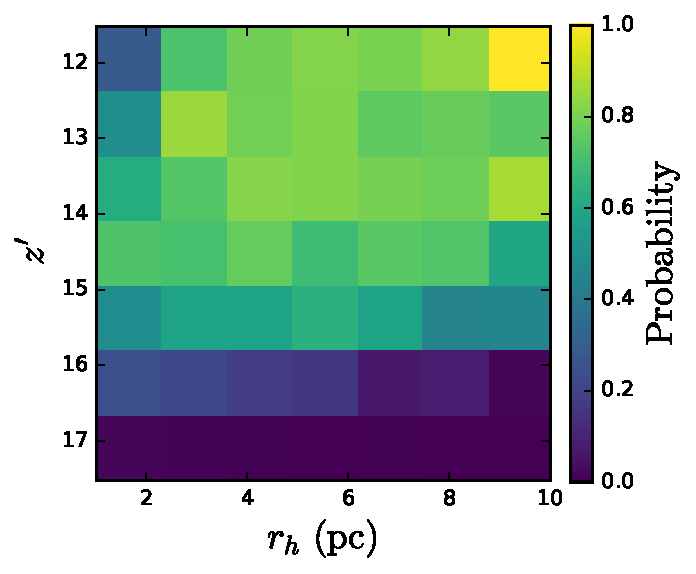
\includegraphics[width=\textwidth]{images/classifier_1.pdf}
	\caption{The probability $P(r_h, m_{z'})$ of correctly classifying an extended object using the initial classifier supplied with data from \textsc{SExtractor}. Classification accuracy decreases as $r_h$ decreases, as the source becomes more pointlike. Similarly, we notice a that objects dimmer than an apparent $z'$ band magnitude of 16.5 are not classified correctly, as they are not detected by \textsc{SExtractor}.The maximum detection rate found corresponds to a $90\%$ chance of detection.}
	\label{fig:comp1}
	\end{minipage}\hfill
	\begin{minipage}[b]{.49\textwidth}
		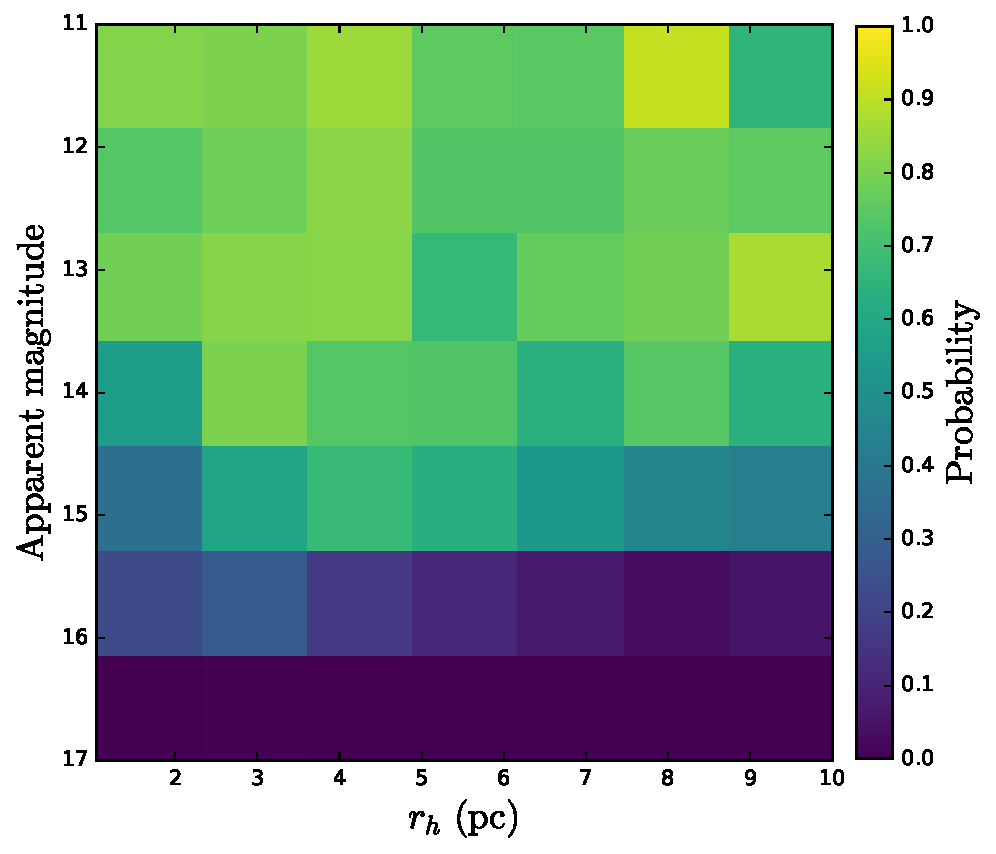
\includegraphics[width=\textwidth]{images/classifier_2.pdf}
		\caption{The probability $P(r_h, \mu)$ of correctly classifying an extended object using the secondary classifier, that is supplied with both data from \textsc{SExtractor} and data from \textsc{IShape} fitting to a King profile. The fitting information allows increased discrimination between point sources and extended objects at lower values of $r_h$. The maximum chance of detection mirrors that found in Figure \ref{fig:comp1} at $90\%$. Detection rates to not increase furthr as the limiting factor becomes \textsc{SExtractor}'s detection and not the classifier.}
		\label{fig:comp2}
	\end{minipage}
\end{figure*}

%
%
%\begin{figure}
%	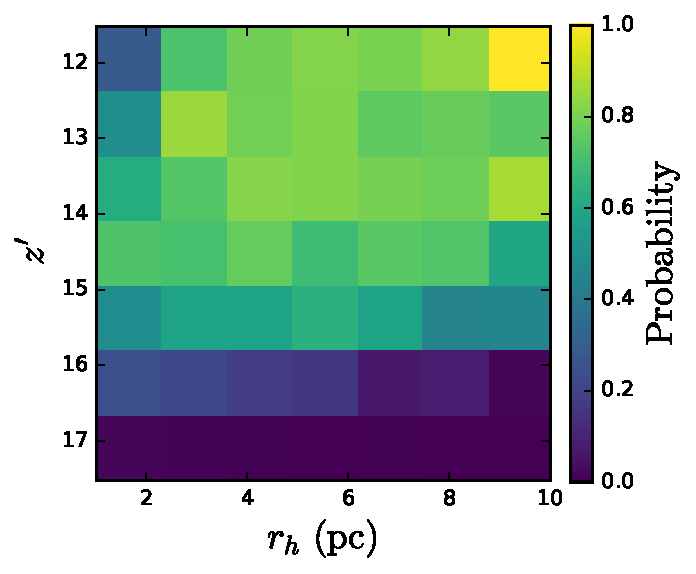
\includegraphics[width=0.49\textwidth]{images/classifier_1.pdf}
%	\caption{The probability $P(r_h, m_{z'})$ of correctly classifying an extended object using the initial classifier supplied with data from \textsc{SExtractor}. Classification accuracy decreases as $r_h$ decreases, as the source becomes more pointlike. Similarly, we notice a that objects dimmer than an apparent $z'$ band magnitude of 16.5 are not classified correctly, as they are not detected by \textsc{SExtractor}.The maximum detection rate found corresponds to a $90\%$ chance of detection.}
%	\label{fig:comp1}
%\end{figure}
%\begin{figure}
%	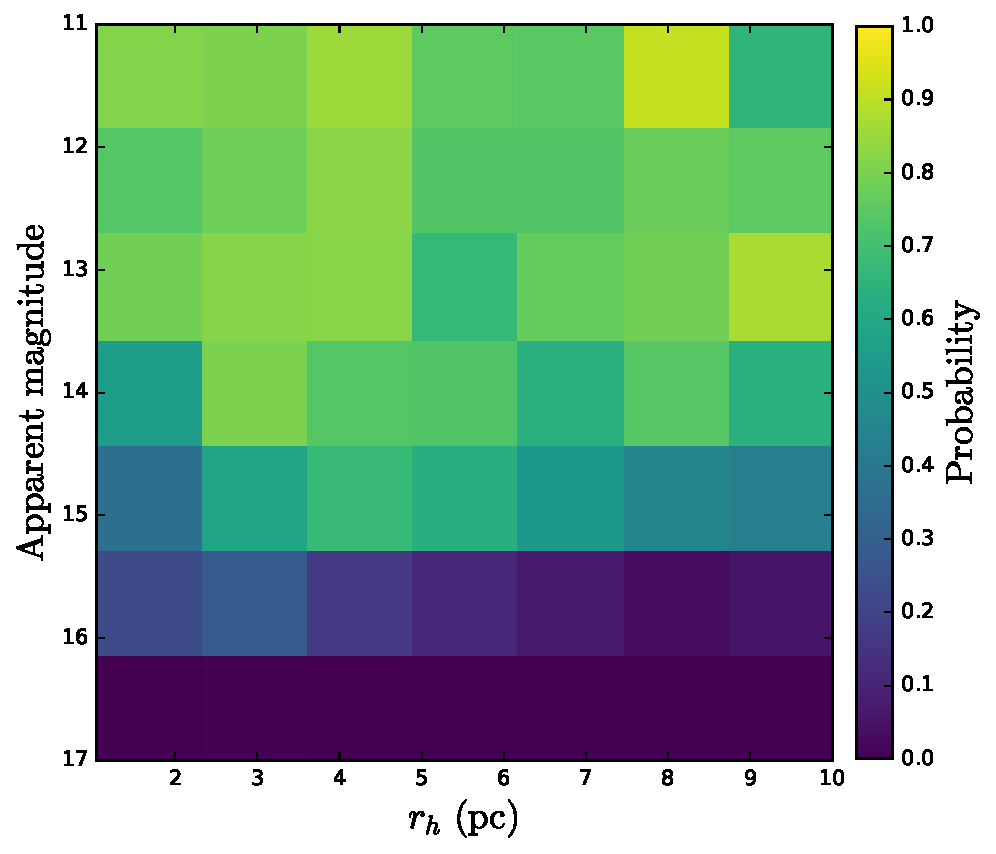
\includegraphics[width=0.49\textwidth]{images/classifier_2.pdf}
%	\caption{The probability $P(r_h, \mu)$ of correctly classifying an extended object using the secondary classifier, that is supplied with both data from \textsc{SExtractor} and data from \textsc{IShape} fitting to a King profile. The fitting information allows increased discrimination between point sources and extended objects at lower values of $r_h$. The maximum chance of detection mirrors that found in Figure \ref{fig:comp1} at $90\%$.}
%	\label{fig:comp2}
%\end{figure}



Each candidate underwent aperture photometry on the fully reduced mosaics mentioned in Section \ref{sec:obs}, where colour magnitude corrections were performed by interpolating the dust maps from \citet{Schlegel1998} and applying the band extinction to redding ratios from \citet{Schlafly2011}. Magnitude calibration was performed by using the Landolt set of standard stars \citep{Landolt1992} that had been transformed via the equations given in \citet{Fukugita1996} into the SDSS system. Zero point magnitude calibrations were determined using the \verb|fitparams| task in \textsc{iraf}.

Further pruning of the globular cluster candidates was performed removing unphysical outliers in the analysis, such as removing objects with a detected fwhm of over a ten arcseconds. In addition, ellipticity cutoffs, colour profile cuts and magnitude cuts were introduced to remove galaxies in the globular cluster candidate list. 


\subsection{Globular clusters color-magnitude diagram}
\label{sec:gc_cmd}

\begin{figure*}
	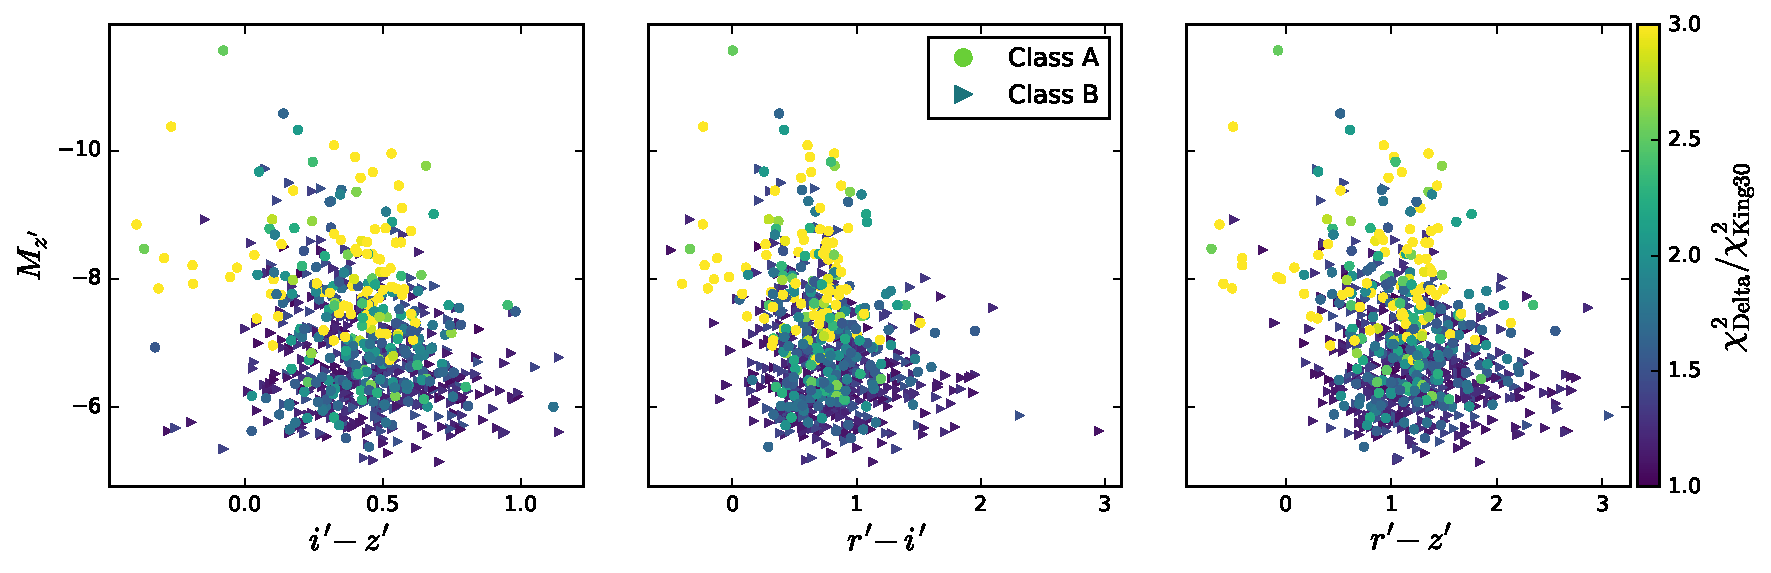
\includegraphics[width=\textwidth]{images/colour.pdf}
	\caption{The determine colours of the GC candidates in the $r'$, $i'$ and $z'$ bands when applicable.{\color{red} put something interesting here} }
	\label{fig:colour}
\end{figure*}

\lipsum[1-2]

\subsection{Globular cluster sizes}
\label{sec:gc_sizes}
\begin{figure}
	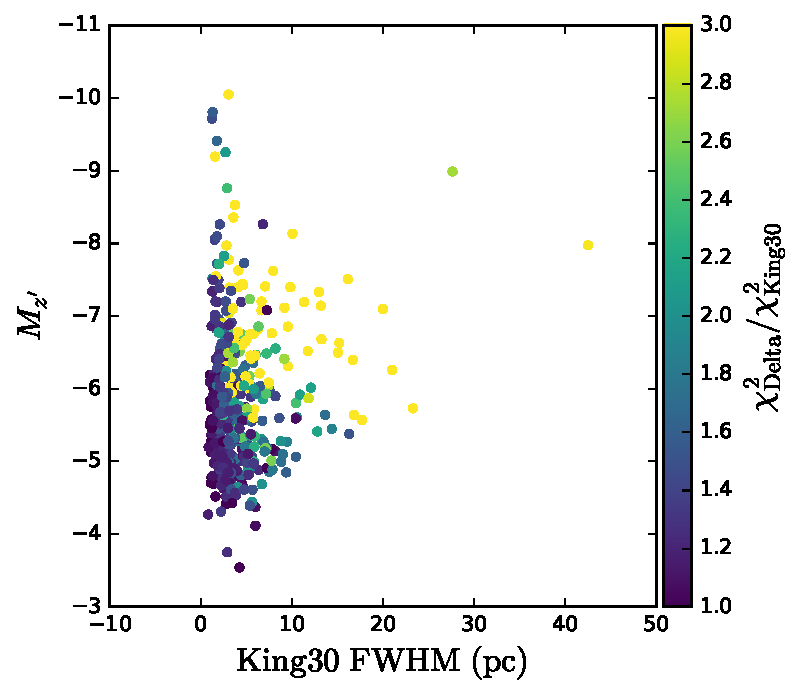
\includegraphics[width=\columnwidth]{images/kingFWHM.pdf}
	\caption{The fitted FWHM of a King30 profile for each GC candidate. Pixel values were transformed into parsecs using a galactic distance of 2.7 Mpc. Brighter and more extended objects have better fits to the King 30 profile than a delta profile, as expected.}
	\label{fig:kfwhm}
\end{figure}

\lipsum[1-2]

%%%%%%%%%%%%%%%%%%%%%%%%%%%%%%%%%%%%%%%%%%%%%%%%%%%%%%%%%%%%%%%%%%%%%%
\section{Discussion}
\label{sec:discussion}

\lipsum[1-2]

%%%%%%%%%%%%%%%%%%%%%%%%%%%%%%%%%%%%%%%%%%%%%%%%%%%%%%%%%%%%%%%%%%%%%%
\section{Summary and conclusions}
\label{sec:conclusions}

\lipsum[1-2]
%%%%%%%%%%%%%%%%%%%%%%%%%%%%%%%%%%%%%%%%%%%%%%%%%%%%%%%%%%%%%%%%%%%%%%%%

\section*{Acknowledgments}

AJR was supported by National Science Foundation grants AST-0808099
and AST-0909237.

\bibliographystyle{mn2e}
\bibliography{maffei1}

\appendix
\onecolumn
\section{Globular cluster candidates photometry}
\label{sec:appendix}



\lipsum[1]



\begin{table}
 \centering
 \caption{Photometry of the first ten ``Class A'' (see main text for its definition) globular cluster candidates. Absolute magnitudes have been computed using $D = 2.7\,\rm{Mpc}$.}
\label{tab:class_a}  
\begin{tabular}{lllccccc}
	\hline
	ID & RA & DEC & $\epsilon$ & $M_{z'}$ & $m_{z'}$ & $r'-z'$ & King$_{30}$ FWHM (pc) \\
	\hline
	A1 & $2^{\rm{h}}\,38^{\rm{m}}\,8.8^{\rm{s}}$ & $59^\circ\,52'\,29.39''$ & 0.10 & -7.399 & 19.757 & 1.473 & 4.88 \\
	A2 & $2^{\rm{h}}\,38^{\rm{m}}\,12.9^{\rm{s}}$ & $59^\circ\,52'\,0.73''$ & 0.07 & -8.487 & 18.670 & 1.363 & 7.04 \\
	A3 & $2^{\rm{h}}\,37^{\rm{m}}\,56.5^{\rm{s}}$ & $59^\circ\,51'\,57.60''$ & 0.25 & -8.708 & 18.449 & 1.411 & 4.10 \\
	A4 & $2^{\rm{h}}\,38^{\rm{m}}\,36.6^{\rm{s}}$ & $59^\circ\,51'\,36.72''$ & 0.17 & -7.123 & 20.033 & 1.004 & 3.64 \\
	A5 & $2^{\rm{h}}\,38^{\rm{m}}\,10.6^{\rm{s}}$ & $59^\circ\,50'\,18.02''$ & 0.20 & -7.194 & 19.963 & 1.282 & 3.84 \\
	A6 & $2^{\rm{h}}\,38^{\rm{m}}\,10.7^{\rm{s}}$ & $59^\circ\,50'\,1.18''$ & 0.24 & -8.158 & 18.999 & 1.412 & 6.64 \\
	A7 & $2^{\rm{h}}\,38^{\rm{m}}\,37.2^{\rm{s}}$ & $59^\circ\,49'\,41.20''$ & 0.10 & -7.116 & 20.041 & 1.512 & 5.48 \\
	A8 & $2^{\rm{h}}\,38^{\rm{m}}\,37.0^{\rm{s}}$ & $59^\circ\,49'\,37.06''$ & 0.16 & -6.685 & 20.471 & 1.458 & 10.54 \\
	A9 & $2^{\rm{h}}\,38^{\rm{m}}\,27.5^{\rm{s}}$ & $59^\circ\,49'\,23.63''$ & 0.17 & -8.271 & 18.886 & 1.114 & 11.32 \\
	A10 & $2^{\rm{h}}\,38^{\rm{m}}\,49.2^{\rm{s}}$ & $59^\circ\,48'\,49.93''$ & 0.11 & -8.477 & 18.680 & 0.919 & 9.81 \\
	A11 & $2^{\rm{h}}\,38^{\rm{m}}\,43.5^{\rm{s}}$ & $59^\circ\,48'\,17.57''$ & 0.18 & -7.249 & 19.908 & 1.412 & 4.85 \\
	A12 & $2^{\rm{h}}\,38^{\rm{m}}\,23.4^{\rm{s}}$ & $59^\circ\,47'\,12.30''$ & 0.12 & -9.437 & 17.720 & 1.070 & 3.55 \\
	A13 & $2^{\rm{h}}\,38^{\rm{m}}\,47.9^{\rm{s}}$ & $59^\circ\,46'\,28.99''$ & 0.18 & -7.695 & 19.461 & 1.290 & 3.81 \\
	A14 & $2^{\rm{h}}\,38^{\rm{m}}\,13.2^{\rm{s}}$ & $59^\circ\,46'\,22.37''$ & 0.20 & -7.492 & 19.665 & 0.958 & 3.35 \\
	A15 & $2^{\rm{h}}\,38^{\rm{m}}\,50.4^{\rm{s}}$ & $59^\circ\,46'\,6.46''$ & 0.19 & -7.094 & 20.063 & 1.673 & 12.07 \\
	\hline
\end{tabular}
\end{table}


\begin{table}
 \centering
  \caption{Photometry of the first ten ``Class B'' globular cluster candidates. Absolute magnitudes have been computed using $D = 2.7\,\rm{Mpc}$.}
\label{tab:class_b}  
\begin{tabular}{lllccccc}
	\hline
	ID & RA & DEC & $\epsilon$ & $M_{z'}$ & $m_{z'}$ & $r'-z'$ & King$_{30}$ FWHM (pc) \\
	\hline
	B1 & $2^{\rm{h}}\,38^{\rm{m}}\,21.8^{\rm{s}}$ & $59^\circ\,54'\,6.98''$ & 0.07 & -9.131 & 18.026 & 0.542 & 1.50 \\
	B2 & $2^{\rm{h}}\,38^{\rm{m}}\,31.3^{\rm{s}}$ & $59^\circ\,53'\,26.38''$ & 0.22 & -8.419 & 18.738 & 1.104 & 1.24 \\
	B3 & $2^{\rm{h}}\,38^{\rm{m}}\,13.0^{\rm{s}}$ & $59^\circ\,53'\,23.32''$ & 0.13 & -6.913 & 20.244 & 0.917 & 0.95 \\
	B4 & $2^{\rm{h}}\,37^{\rm{m}}\,60.0^{\rm{s}}$ & $59^\circ\,53'\,6.65''$ & 0.23 & -6.219 & 20.938 & 0.806 & 8.14 \\
	B5 & $2^{\rm{h}}\,38^{\rm{m}}\,23.3^{\rm{s}}$ & $59^\circ\,52'\,56.42''$ & 0.08 & -6.236 & 20.921 & 1.711 & 1.91 \\
	B6 & $2^{\rm{h}}\,38^{\rm{m}}\,6.6^{\rm{s}}$ & $59^\circ\,52'\,39.65''$ & 0.10 & -5.960 & 21.197 & 0.989 & 6.32 \\
	B7 & $2^{\rm{h}}\,37^{\rm{m}}\,57.0^{\rm{s}}$ & $59^\circ\,52'\,25.79''$ & 0.19 & -6.163 & 20.993 & 1.074 & 3.35 \\
	B8 & $2^{\rm{h}}\,38^{\rm{m}}\,54.5^{\rm{s}}$ & $59^\circ\,51'\,57.06''$ & 0.18 & -8.274 & 18.882 & 1.369 & 4.42 \\
	B9 & $2^{\rm{h}}\,38^{\rm{m}}\,20.6^{\rm{s}}$ & $59^\circ\,51'\,57.31''$ & 0.02 & -7.098 & 20.059 & 2.321 & 1.33 \\
	B10 & $2^{\rm{h}}\,38^{\rm{m}}\,33.8^{\rm{s}}$ & $59^\circ\,50'\,17.84''$ & 0.20 & -6.527 & 20.629 & 2.443 & 1.39 \\
	B11 & $2^{\rm{h}}\,38^{\rm{m}}\,45.9^{\rm{s}}$ & $59^\circ\,48'\,36.76''$ & 0.22 & -7.152 & 20.005 & 0.921 & 3.72 \\
	B12 & $2^{\rm{h}}\,38^{\rm{m}}\,57.7^{\rm{s}}$ & $59^\circ\,48'\,33.88''$ & 0.12 & -6.630 & 20.527 & 2.544 & 1.47 \\
	B13 & $2^{\rm{h}}\,38^{\rm{m}}\,39.6^{\rm{s}}$ & $59^\circ\,45'\,45.43''$ & 0.15 & -6.093 & 21.063 & 0.824 & 2.48 \\
	B14 & $2^{\rm{h}}\,38^{\rm{m}}\,38.3^{\rm{s}}$ & $59^\circ\,44'\,16.26''$ & 0.05 & -6.608 & 20.548 & 1.524 & 2.74 \\
	B15 & $2^{\rm{h}}\,38^{\rm{m}}\,42.5^{\rm{s}}$ & $59^\circ\,43'\,56.03''$ & 0.05 & -6.416 & 20.741 & 2.649 & 3.72 \\
	\hline
\end{tabular}
\end{table}


%\lipsum[1]

%\bsp
\label{lastpage}

\end{document}
